\begin{enunciado}{\ejercicio}
  Se define la siguiente relación $\relacion$ en $G_{20}$:
  $$
    z\relacion w \sisolosi zw^9 \en G_2.
  $$
  \begin{enumerate}[label=\roman*)]
    \item Probar que $\relacion$ es una relación de equivalencia.
    \item Calcular la cantidad de elementos que hay en cada clase de equivalencia.
  \end{enumerate}
\end{enunciado}

\begin{enumerate}[label=\roman*)]
  \item
        \textit{Reflexividad: }
        $$
          z = e^{i\frac{1}{10}\pi k_z}
          \entonces
          z \relacion z
          \sisolosi
          e^{i\frac{1}{10}\pi k_z} \cdot e^{i\frac{9}{10}\pi k_z} =
          e^{ik_z\pi } =
          \llave{rl}{
            1 & k_z \text{ par}\\
            -1 & k_z \text{ impar}
          } \Tilde
        $$

        \textit{Simetría: }
        La relación $\relacion$ será simétrica si:
        $$
          z \relacion w
          \sisolosi w \relacion z
        $$
        De forma exponencial para poder expresar el producto de un número por otro:
        $$
          z = e^{i\frac{1}{10}\pi k_z} \en G_{20}
          \ytext
          w = e^{i\frac{1}{10}\pi k_w} \en G_{20}.
        $$
        $$
          zw^9 = e^{i \frac{\pi}{10}(k_z + 9k_w)} \en G_2
          \sii
          \frac{1}{10}(k_z + 9k_w) = k
          \sii
          k_z + 9k_w = 10k
          \sii
          \congruencia{k_z}{-9k_w}{10}
        $$
        Quedando la dentro de todo simpática relación de congruencia que me permite reescribir la definición de la relación:
        $$
          \congruencia{k_z}{k_w}{10}
          \Sii{\red{!}}
          \boxed{
            z\relacion w
            \sisolosi
            \congruencia{k_z}{k_w}{10}
          }
        $$
        Voy a expresar ahora $w \relacion z$:
        $$
          wz^9 = e^{i \frac{\pi}{10}(k_w + 9\magenta{k_z})} =
          e^{i \frac{\pi}{10}(k_w + 9(\magenta{10k + k_w}))} =
          e^{i \frac{\pi}{10}(90k + 10k_w)} =
          e^{i (9k + k_w)\pi} =
          e^{i\blue{k'}\pi}
          \text{ con } \blue{k'} \en \enteros \\
        $$
        Por lo tanto se puede concluír que la relación es simétrica
        $\paratodo k_z,\,k_w \en \enteros \text{ con } \congruencia{k_z}{k_w}{10}$

        \textit{Transitividad: }

        $$ \llaves{l}{
            z = e^{i\frac{1}{10}\pi k_z}\\
            w = e^{i\frac{1}{10}\pi k_w}\\
            y = e^{i\frac{1}{10}\pi k_y}
          } \en G_{20}
        $$
        Entonces la relación $\relacion$ es transitiva si:
        $$
          z \relacion w  \ytext w\relacion y
          \Entonces{atajo}
          z \relacion y
        $$
        Del punto anterior sé que:
        $$
          \llave{l}{
            z \relacion w
            \sisolosi
            \congruencia{k_z}{k_w}{10} \llamada1\\
            w \relacion y
            \sisolosi
            \congruencia{k_w}{k_y}{10} \llamada2
          }
        $$
        Planteo similar al punto anterior, veo que cosa queda del producto:
        $$
          zy^9 = e^{i \frac{\pi}{10}(\magenta{k_z} + 9k_y)}
          \igual{$\llamada 1$}
          e^{i \frac{\pi}{10}(\magenta{10 \blue{k} + k_w} + 9k_y)}
          \igual{$\llamada 2$}
          e^{i \frac{\pi}{10}(10 \blue{k} + 10\blue{k'} + k_y + 9k_y)}
          \igual{\red{!}}
          e^{i (k + k' + k_y) \pi}  =
          e^{i \blue{k''} \pi}
        $$
        Con ese resultado podemos concluir que la relación es transitiva:
        $$
          z \relacion w
          \ytext
          w \relacion z
          \entonces z\relacion y
        $$

        Dado que la relación $\relacion$ resultó ser \textit{reflexiva}, \textit{simétrica} y \textit{transitiva}, es
        también una relación de \textit{equivalencia}.

  \item $\# \clase{e^{i\frac{2\pi}{20} k}} = 2$ para algún $k \en \enteros / r_{20}(k) < 20$. Dada
        la condición $\congruencia{k_z}{k_w}{10}$, solo hay 2 números que tienen misma cifra de unidad
        entre 0 y 20. En el gráfico se ve que si $z\relacion w \entonces w = -z $
\end{enumerate}
$$
  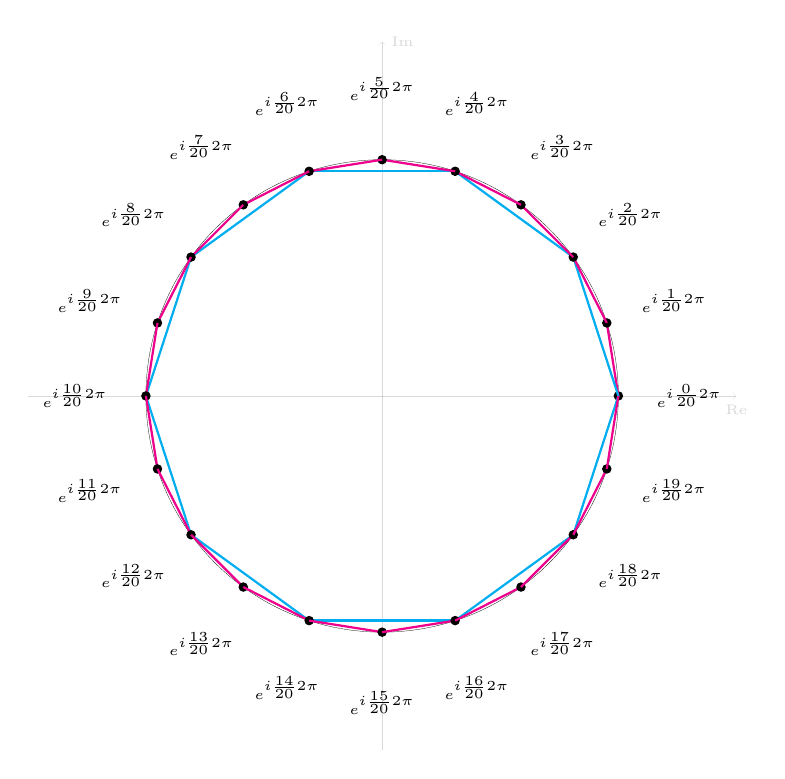
\begin{tikzpicture}[baseline=0,scale = 3, every node/.style={font=\tiny}]
    \draw[ultra thin,->,gray, opacity=0.3] (-1.5,0) -- (1.5,0) node[below] {Re};
    \draw[ultra thin,->,gray, opacity=0.3] (0,-1.5) -- (0,1.5) node[right] {Im};
    \draw[ultra thin] (0,0) circle (1);
    \foreach \x in {0,...,19} {
        \filldraw (\x*360/20:1) circle (0.5pt);
        \filldraw (\x*360/20:1.3) node { $e^{i\frac{\x}{20}2\pi}$};
        \ifnum\x<20
          \draw[thick, magenta] (\x*360/20:1) -- ({(\x+1)*360/20}:1);
        \fi
        \ifnum\x<10
          \draw[thick, cyan] (\x*360/10:1) -- ({(\x+1)*360/10}:1);
        \fi
      }
  \end{tikzpicture}
$$

\begin{aportes}
  \item \aporte{\dirRepo}{naD GarRaz \github}
\end{aportes}
